\section{Lossless acceleration}
\label{sec:accel}

\begin{figure*}[t]
\centering
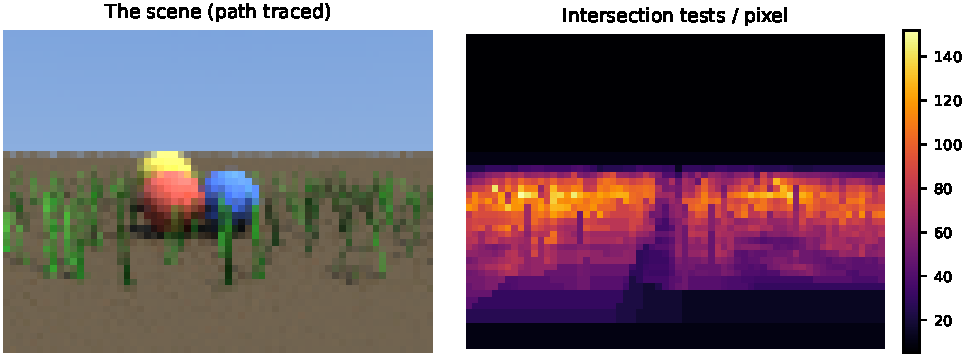
\includegraphics[width=\textwidth]{figures/scene_cost.pdf}
\caption{Left: the canonical scene, path traced. Right: intersection tests per
pixel for a primary-plus-shadow ray. The grass dominates the cost budget ---
exactly the geometry the lossless tricks target.}
\label{fig:scene}
\end{figure*}

\begin{figure*}[t]
\centering
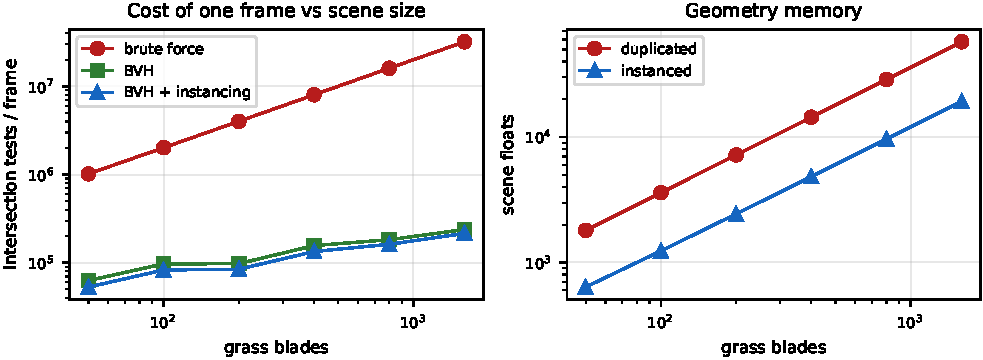
\includegraphics[width=\textwidth]{figures/accel_scaling.pdf}
\caption{Left: intersection tests to render one frame as the grass field grows.
Brute force is linear in triangle count; the BVH and instancing are far flatter.
Right: geometry memory --- instancing stores one blade plus per-instance
transforms instead of duplicated triangles.}
\label{fig:accel}
\end{figure*}

Figure~\ref{fig:scene} shows where a frame's cost goes: the per-pixel test count
is concentrated on the grass, which is why accelerating grass is the whole game.
Both lossless methods produce an image \emph{identical} to brute force --- we
verify bit-for-bit equality in the unit tests (BVH versus brute; instancing
versus duplicated geometry) --- so their only effect is on the test count.

\paragraph{BVH.} Brute force tests every ray against every triangle, and
Figure~\ref{fig:accel} (left) shows the resulting linear growth: on our largest
field (\BigBlades\ blades, \BigTris\ triangles) a primary-plus-shadow pass costs
\BruteTestsBig\ tests. The BVH cuts this to \BvhTestsBig, a
\AccelSpeedup$\times$ reduction, and the gap widens with scene size because the
BVH cost grows roughly logarithmically in the number of primitives. On the
smaller rendered scene the lossless BVH speedup is \BvhSpeedupRender$\times$; the
factor is not a constant but a function of how much geometry the structure lets
each ray skip.

\paragraph{Instancing.} Instancing adds a second win. In test count it edges out
the flat BVH (\AccelSpeedupInst$\times$ versus \AccelSpeedup$\times$ on the large
scene) because the shared blade BVH is tiny and cache-friendly to traverse. Its
real advantage, though, is memory: Figure~\ref{fig:accel} (right) contrasts
storing $K$ duplicated blades against one blade plus $K$ cheap transforms. With
our deliberately tiny four-triangle blade the memory ratio is only
\MemRatio$\times$, because a $3\times3$-plus-translation transform ($12$ floats)
is not much smaller than four triangles ($36$ floats); the ratio grows towards
the blade's triangle count for realistic vegetation with hundreds of triangles
per blade. This is the honest shape of the grass trick: for the geometry Nintendo
was drawing, instancing turns a prohibitive memory footprint into a trivial one,
and it does so for free in image quality.

The lesson of this section is that a large part of ray tracing's cost is simply
\emph{waste} --- testing rays against geometry they could never hit --- and that
removing it changes nothing about the picture. Only after this free lunch do real
trade-offs begin.
